\documentclass[main.tex]{subfiles}
\begin{document}
% 5,  part 2
\begin{psec}{5.20}%
Next,
we look at some properties of the square root map.
\begin{enumerate}
\item \label{5.20-1} \statement{
Let $S\in\mathscr{H}$, $T\in{\mathscr H}^+$.
If $S$ commutes with~$T$,
then it commutes with~$\sqrt{T}$.}
This follows from the last part of~\ref{5.19}:
$S$ commutes with all powers of~$T$,
therefore with every $\sr_n(T)$,
therefore with~$\sqrt{T}$.
%
\item \label{5.20-2} \statement{
If $S,T\in\mathscr{H}^+$ and $ST=TS$, then $ST\in{\mathscr H}^+$.}

\noindent \emph{Proof}\  By~\ref{5.12}, $ST\in{\mathscr H}$.
As for the positivity: 
\ref{5.20-1} implies that~$T$ commutes with~$\sqrt{S}$
and, again, that~$\sqrt{S}$ commutes with~$\sqrt{T}$.
Then $ST=\smash{\sqrt{S}^2} \smash{\sqrt{T}^2}
= \smash{\bigl(\sqrt{S}^{\phantom{2}}\sqrt{T}\,\bigr)^2}\in{\mathscr H}^+$
\quad(\ref{5.9}). \xqed
%
\item \label{5.20-3} \statement{
Let $S,T\in\mathscr{H}$, $S\leq T$.
Then $VS\leq VT$ for every~$V$ in~${\mathscr H}^+$
that commutes with~$S$ and with~$T$.}

\noindent \emph{Proof}\  $VS-VT=V(T-S)\in{\mathscr H}^+$,
by~\ref{5.20-2}. \xqed
%
\item \label{5.20-4} \statement{
Let $S,T\in{\mathscr H}^+$, $ST=TS$.
If $S\leq T$, then $S^2 \leq T^2$.}

\noindent \emph{Proof}\ With~\ref{5.20-3}:
$SS\leq ST=TS\leq TT$. \xqed
%
\item \label{5.20-5} \statement{
Let $T\in{\mathscr H}^+$, $V\in\mathscr H$, $TV=VT$.
If $V^2\leq T$, then $V\leq \sqrt{T}$.}

\noindent\emph{Proof}\  We may assume $\|T\|=1$.
Let~$q_n$ be as in~\ref{5.18} and~\ref{5.19},
so that $q_n(I-T)\rightarrow I-\sqrt{T}$.
We are done if $q_n(I-T)\leq I-V$ for all~$n$.
This inequality can be proved inductively.
First: 
\begin{alignat*}{2}
I-V-q_1(I-T) 
& = I-V-{\textstyle \frac{1}{2}}(I-T)  & \\
& = {\textstyle \frac{1}{2}} I - V + {\textstyle \frac{1}{2}} T & \\
& \geq {\textstyle \frac{1}{2}} I - V + {\textstyle \frac{1}{2}} V^2
 &= {\textstyle \frac{1}{2}} (I-V)^2 \geq 0\htam{,}
\end{alignat*}
so $q_1(I-T)\leq I-V$.

Second:  if~$n$ is so that $q_n(I-T)\leq I-V$, then
\begin{alignat*}{2}
2q_{n+1} (I-T) 
& = I-T+(q_n(I-T))^2 & \\
& \relref{\leq}{5.20-4} I-T+(I-V)^2 & \\
& \leq I-V^2+(I-V)^2 & = 2(I-V)
\end{alignat*}
and $q_{n+1} (I-T) \leq I-V$. \xqed
%
\item \label{5.20-6} \statement{
If $T\in{\mathscr H}^+$, then $\smash{\sqrt{T^2}=T}$.}

\noindent \emph{Proof} Put $S:=\smash{\sqrt{T^2}}-T$.
By~\ref{5.20-5}, $T\leq \smash{\sqrt{T^2}}$,
i.e., $S\geq 0$.
Then $ST\geq 0$ according to~\ref{5.20-2}.
But~$ST$ equals $-\frac{1}{2} S^2$.
Hence for all~$x$ in~$H$
\begin{equation*}
\|Sx\|^2 = \left<Sx,Sx\right>=\left<S^2 x,x\right>
=-2\left<STx,x\right>\leq 0\htam{.}
\end{equation*}
It follows that $S=0$, and $\smash{\sqrt{T^2}}=T$. \xqed
\end{enumerate}
\end{psec}
%
%                  5.21
%
\begin{psec}{5.21}{Exercise}
Let $S,T\in{\mathscr H}^+$ be so that $\|Sx\|=\|Tx\|\quad(x\in H)$.
Prove $S=T$.
(Show first that $S^2 = T^2$.)
\end{psec}
%
%                  5.22
%
\begin{psec}{5.22}{Exercise}
(This we need farther on.)
Prove the following.
\begin{enumerate}
\item\label{5.22-1}
If $T\in\mathscr H$ and $0\leq T\leq I$, then $T^2\leq T$.
%
\item\label{5.22-2}
If $T\in\mathscr H$ and $0\leq T\leq I$,
then $\|Tx\|^2\leq \left< Tx,x\right>\quad (x\in H)$.
%
\item\label{5.22-3}
If $S,T\in\mathscr H$ and $0\leq S\leq T\leq I$,
then 
\begin{equation*}
\|Tx-Sx\|^2 \leq \left<Tx,x\right>-\left<Sx,x\right>\qquad (x\in H)\htam{.}
\end{equation*}
\end{enumerate}
\end{psec}
%
%                  5.23
%
\begin{psec}{5.23}{Exercise}
(built upon the previous one)
Let $T\in\mathscr H$, $0\leq T\leq I$
(or: $T\in{\mathscr H}^+$, $\|T\|\leq 1$).
Prove:
\begin{enumerate}
\item\label{5.23-1}
$I\geq T \geq T^2 \geq \dotsb$.
%
\item\label{5.23-2}
$Px:=\lim_{n\ra\infty} T^n x$ exists for all~$x$ in~$H$.

This defines a (linear) map $P\colon H\ra H$.
For each~$x$ in~$H$
we see that $\|x\|\geq\|Tx\|\geq\|T^2 x\|\geq \dotsb$,
so that $\|Px\|\leq \|x\|\quad (x\in H)$
and~$P$ is continuous.
%
\item\label{5.23-3}
$P\in\mathscr H$, $0\leq P \leq T\leq I$.
%
\item\label{5.23-4}
$P=P^2$. (Careful: From $T^n x\ra Px\quad(x\in H)$
it does not immediately follow that $T^{2n} x\ra P^2 x\quad(x\in H)$.
Instead, prove $\left<Px,x\right>=\|Px\|^2$.)

Thus, $P$ is a projection (\ref{5.7}).
%
\item\label{5.23-5}
If $x\in H$ and $Tx=x$,
then $Px=x$.
Conversely,
if $x\in H$ and $Px=x$,
then $\left< Tx,x\right>=\left<x,x\right>$,
so $Tx-x\perp x$,
whence $Tx=x$ (Pythagoras).

$P$ is the projection onto $\left\{ x\colon Tx=x \right\}$.
\end{enumerate}
\end{psec}
%
%                  5.24
%
\begin{psec}{5.24}{Exercise}
(built upon the previous one)
\begin{center}
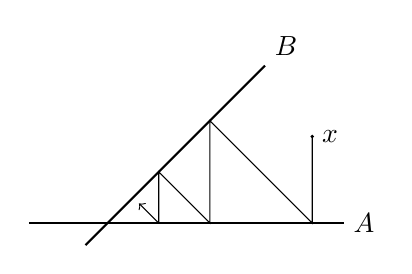
\begin{tikzpicture}
% A:
\draw[line width=.8pt] (-1,0) -- (3,0);
\draw (3,0) node[anchor=west]{$A$};

% B:
\draw[line width=.8pt] (-.28,-.28) -- (2,2);
\draw (2,2) node[anchor=south west]{$B$};

% x:
\draw[fill=black] (2.6,1.1) circle (.4pt);
\draw (2.6,1.1) node[anchor=west]{$x$};

% projections:
\draw (2.6,1.1) -- (2.6,0) -- (1.3,1.3) -- (1.3,0) -- (.65,.65) -- (.65,0);
\draw[->] (.65,0) -- (.4,.25);
\end{tikzpicture}
\end{center}
Let~$A$ and~$B$ be closed linear subspaces of~$H$
with projections~$Q$ and~$R$, respectively.
We consider the sequence
\begin{equation*}
Q,\ RQ,\ QRQ,\ RQRQ,\ \dotsc
\end{equation*}
Prove the following.
\begin{enumerate}
\item\label{5.24-1}
$QRQ\in\mathscr H$, $0\leq QRQ \leq I$.
%
\item\label{5.24-2}
For all $x\in H$ the sequence $QRQx$,  $QRQRQx$, 
$\dotsc$ converges.

Denote its limit by~$Px$.
We now have a map $P\colon H\ra H$.
%
\item\label{5.24-3}
$P$ is the projection onto $A\cap B$.
(If $QRQx=x$, then $x\in Q(H)$, so $Qx=x$.)
%
\item\label{5.24-4}
For every~$x$ the sequence
\begin{equation*}
Qx,\ RQx,\ QRQx,\ RQRQx,\ \dotsc
\end{equation*}
converges to~$Px$.
\end{enumerate}
\end{psec}

\noindent
We begin to get results:
\begin{psec}{5.25}{Lemma}\statement{
Let $\mathscr A$ be a closed subalgebra of~$\mathscr H$.
\begin{enumerate}
\item\label{5.25-1} $\mathscr A$ is a Riesz space
under the ordering of~$\mathscr H$, and 
\begin{equation*}
|T|\ =\ \sqrt{T^2}\qquad(T\in\mathscr A)\htam{.}
\end{equation*}
%
\item\label{5.25-2} If $I\in\mathscr A$,
then~$I$ is a unit,
the norm~$\|\cdot\|_I$ is the operator norm,
and~$\mathscr A$ is uniformly complete.
\end{enumerate}
}\end{psec}
\begin{proof}
\begin{enumerate}
\item
It suffices to prove that for $T\in \mathscr A$,
$\smash{\sqrt{T^2}}$ is the supremum of $\{T,-T\}$
in the ordered vector space~$\mathscr A$.
Let $T\in\mathscr A$.
\begin{itemize}
\item  In the final lines of~\ref{5.19}
we have seen that $\sqrt{T}\in\mathscr A$,
\item $\pm T \leq \smash{\sqrt{T^2}}$, 
since $(\pm T)^2\leq T^2$ (\ref{5.20}\ref{5.20-5}).
\item Let $W$ be an upper bound of $\{T,-T\}$ in~$\mathscr A$.
Then $W\geq \frac{1}{2}(T+-T)=0$.
Also, with~\ref{5.20}\ref{5.20-2}, 
$0\leq (W-T)(W+T)=W^2-T^2$,
so that $W^2\geq T^2$ and,
with~\ref{5.20}\ref{5.20-6} and~\ref{5.20}\ref{5.20-5},
$W=\smash{\sqrt{W^2}}\geq\smash{\sqrt{T^2}}$.
\end{itemize}
%
\item \label{5.25-2}
For $T\in\mathscr A$
we see that $|T|^2=T^2$.
Then for all~$x$ in~$H$
\begin{equation*}
\| T x \|\ = \|\, |T|x\, \|\htam{,}
\end{equation*}
since
$\|Tx\|^2=\left<Tx,Tx\right>
=\left<T^2x,x\right>
=\left<|T|^2x,x\right>
=\||T|x\|^2$.
Hence, $T$ and~$|T|$
have the same operator norm.
From lemma~\ref{5.20}
it follows easily that~$I$ is a unit in~$\mathscr A$
and that $\|\,|T|\,\|_I$ equals the operator norm of~$|T|$.
Thus, $\|T\|_I=\|T\|$.

As a closed subset of~$\mathscr H$
or~$\Lin(H,H)$,
$\mathscr A$ is complete in the operator norm (\ref{5.1}\ref{5.1-2}),
hence uniformly complete. \xqed
\end{enumerate}
\end{proof}

\noindent The moral is obvious:
By Yosida's Theorem every closed subalgebra of~$\mathscr H$
that contains~$I$
is Riesz isomorphic to some~$\Cont{\Phi}$.
Before filing this result as a theorem
we address ourselves to a question.
Both the operator algebra and~$\Cont{\Phi}$
carry multiplications.
Any connection?

The following lemma paves the way to an affirmative answer.
%
%                  5.26
%
\begin{psec}{5.26}{Lemma}\statement{
Let $E$ be a Riesz space with a unit~$e$.
Suppose there is given a ``multiplication'' 
$*\colon E\times E\ra E$ satisfying
\begin{itemize}
\item For every~$a$ in~$E$
the maps $x\mapsto a*x$ and $x\mapsto x*a$ are linear;
\item $e*a=a*e=a$ for all~$a$ in~$E$;
\item if $a,b\in E^+$,
then $a*b\in E^+$.
\end{itemize}
Let $\varphi\colon E\ra \R$ be a Riesz homomorphism
with $\varphi(e)=1$.
Then $\varphi$ is ``multiplicative'':
\begin{equation*}
\varphi(x*y) \ =\ \varphi(x)\,\varphi(y)\qquad(x,y\in E)\htam{.}
\end{equation*}
}\end{psec}
\begin{proof}
\begin{enumerate}[label=(\Roman*)]
\item\label{5.26-I}
First, an auxiliary formula:
If $a,b\in E$, then
\begin{equation*}
|a*b|\ \leq\ |a|*|b|\htam{.}
\end{equation*}
Indeed,
\begin{alignat*}{2}
|a*b|\ &=\ \bigl|(a^+-a^-)*(b^+-b^-)\bigr| \\
&=\ \bigl| a^+*b^+ \,-\,a^-*b^+ \,-\, a^+*b^- \,+\, a^-*b^- \bigr| \\
&\leq\ \phantom{\bigl|}a^+*b^+ \,+\, a^-*b^+ \,+\, a^+*b^- \,+\,a^-*b^-\\
&=\  (a^+ + a^-)*(b^++b^-) \ =\ |a|*|b|
\end{alignat*}
%
\item\label{5.26-II}
With $a\in E$ and $|a|\leq e$ we get for all $\lambda\in\R$:
\begin{alignat*}{2}
|a*a - \lambda a|
\ &=\ |a*(a-\lambda e)|\ &&\leq\ |a|*|a-\lambda e| \\
\ &\leq\ e*|a-\lambda e|\ &&=\ |a-\lambda e|\htam{,}\intertext{%
and, upon applying $\varphi$:}%
|\varphi(a*a)-\lambda\varphi(a)|\ &\leq\ |\varphi(a)-\lambda|\htam{.}\\%
\intertext{Choosing $\lambda = \varphi(a)$ yields}%
\varphi(a*a)\ &=\ \varphi(a)^2\htam{.}
\end{alignat*}
%
\item\label{5.26-III}
It follows that for \emph{all} $z\in E$,\quad  $\varphi(z*z)=\varphi(z)^2$.
For $x,y\in E$ we have
\begin{equation*}
2\,x*y\ =\ (x+y)*(x+y) \,-\, x*x \,-\, y*y
\end{equation*}
so that
\begin{equation*}
2\,\varphi(x*y)\ 
=\ (\varphi(x)+\varphi(y))^2 - \varphi(x)^2 - \varphi(y)^2
\ =\ 2\,\varphi(x)\,\varphi(y)\htam{,}
\end{equation*}
and we are done. \xqed
\end{enumerate}
\end{proof}
\end{document}
